%
% Architecture
%
\chapter{Architecture}

\minitoc


\section*{Introduction}
Maintenant que tous les composants ont été défini, on peut se pencher plus en détails sur les différents niveaux composant notre logiciel et spécifier comment on passe du modèle architectural au modèle physique. Pour faire cela, on va définir sous quelle forme de tables relationnelles nos classes pourront persister, expliquer les patrons de conceptions que nous avons utilisé dans notre modèle de classes et comment on génère le code à partir de celui-ci.


\section{Architecture physique}

%%Intro
	
Le logiciel lourd que nous écrivons se découpe en différentes couches : 

%% Image

\begin{figure}[htbp]

		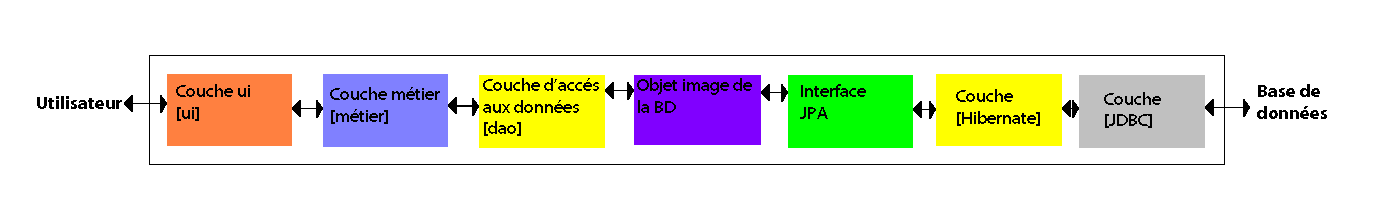
\includegraphics[width=18cm]{images/ArchitecturePhysique.png}
	\caption{Architecture de l'application}
	\label{ArchitectureDeLApplication}
\end{figure}

%% Explication de l'image
%% Ajouter pour chaque couche un exemple de quel code est représenté par cette couche

\begin{enumerate}
\item la couche [ui] (User Interface) est la couche qui dialogue avec l'utilisateur via une interface graphique. Elle a pour rôle de fournir des données provenant de l'utilisateur à la couche [2] ou bien de présenter à l'utilisateur des données fournies par la couche [2].
\begin{itemize}
\item Représente les fenêtres Utilisateur.
\end{itemize}

\item la couche [2], appelée ici [metier] est la couche qui applique les règles dites métier, c.a.d. la logique spécifique de l'application, sans se préoccuper de savoir d'où viennent les données qu'on lui donne, ni où vont les résultats qu'elle produit.
\begin{itemize}
\item Représente les différentes fonctions de notre programme : collecter traiter ...
\end{itemize}

\item la couche [3], appelée ici [dao] (Data Access Object) est la couche qui fournit à la couche [2] des données pré-enregistrées (fichiers, bases de données, ...) et qui enregistre certains des résultats fournis par la couche [2].
\begin{itemize}
\item La couche dao rassemble les descripteurs des classes qui seront "persistées".
\end{itemize}

\item La couche [4] des objets-images de la BD est appelée "contexte de persistance". Elle fait le lien entre la couche [dao] qui s'appuie sur Hibernate pour faire des actions de persistance (CRUD, create - read - update - delete).  Cette couche, fournie par la couche inférieure [5] représente la base de donnée : on n'utilise pas directement la base de données physique.
\begin{itemize}
\item Appellée lors des ajouts suppressions ... sur la base de données.
\end{itemize}

\item L'interface [JPA] est un ensemble générique d'interfaces permettant des accès plus bas niveau (sur les couches physiques comme la base de données) sans avoir à mettre les mains dans le camboui. Elle permet de rendre toutes ses couches inférieures réutilisables.
\begin{itemize}
\item Chaque classe qui doit être "persistée" doit posséder un classe Entity faisant justement partie de la couche JPA.
\end{itemize}

\item La couche [Hibernate] traduit les actions de persistence en ordres SQL.Pour les actions d'interrogation de la base (le SQL Select), Hibernate fournit au développeur, un langage HQL (Hibernate Query Language) pour interroger le contexte de persistance [4] et non la BD elle-même. Cette couche fait le pont entre le monde relationnel et le monde objet.
\begin{itemize}
\item Hibernate est une couche transparente et fourni des outils, et donc n'apparait pas directement dans le code.
\end{itemize}

\item la couche [JDBC] est la couche standard utilisée en Java pour accéder à des bases de données. C'est ce qu'on appelle habituellement le pilote Jdbc du SGBD.
\begin{itemize}
\item Représente la base de données physique.
\end{itemize}

\end{enumerate}

\paragraph*{}
Nous obtenons ainsi une chaîne reliant l'utilisateur (hors logiciel) jusqu'à la base de données (couche la plus physique) contenant ses informations. Chaque couche possède des règles et discute avec les couches l'entourant. Chaque couche modifie ou interprète les informations pour la couche inférieure/supérieure et permet ainsi le fonctionnement du logiciel.


\section{Schémas des bases de données}
	
	\subsection{Logins et mots de passe}

	La base de données des identifiants n'est jamais chargé. Quand un utilisateur entre un mot de passe, le programme chiffre celui-ci et parcourt le fichier pour comparer si le mot de passe chiffré qu'il vient de générer et celui stocké pour cet utilisateur sont les mêmes. Cette opération est simple et ne doit être faite que peu souvent, c'est pourquoi on peut se permettre de ne pas charger le contenu du fichier dans une base de données.

	\subsection{Java Persistence API}
	
	Les comptes sont stockés localement dans des fichiers et lorsque l'utilisateur a entré un mot de passe correct, le programme charge le compte lié à ce mot de passe dans la base de donnée pour y accéder et modifier les informations. C'est ainsi que la persistance est géré pour les comptes hors connexion ou dont la connexion est inactive.
	\paragraph*{}
	Le compte est géré de manière différente selon le programme (classes) et la base de données (tables). On doit donc écrire des schémas de "traduction" de la base de données relationnelle aux classes. Nous avons choisi de créer une table par chemin d'héritage.
	\paragraph*{}
	On commence en réalisant les schémas de toutes les classes isolées (ne dépendant pas de chemins d'héritage) :\\

	\begin{figure}[htbp]

		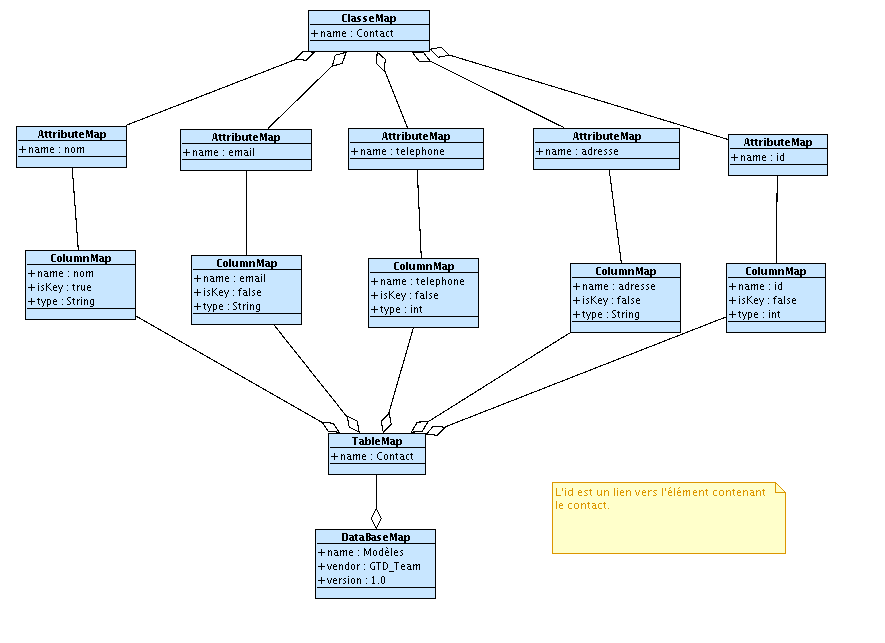
\includegraphics[width=18cm]{images/L4/ContactDBS.png}
	\caption{Schéma de la base de données : Table Contacts}
	\label{ContactDBS}
\end{figure}
La table "Contact" \ref{ContactDBS} contient les colonnes liées aux attributs de la classe associée, plus l'id de la tâche, du projet ou directement du compte auquel elle est liée. \\


\begin{figure}[htbp]

		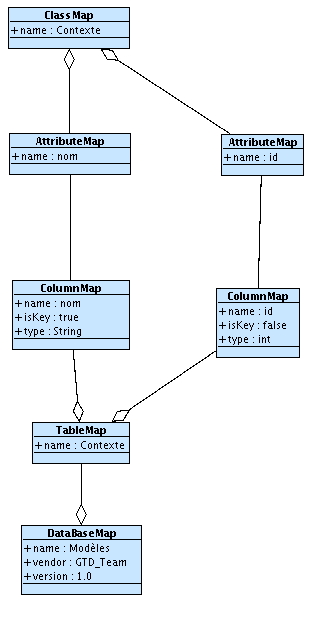
\includegraphics[width=10cm]{images/L4/ContexteDBS.png}
	\caption{Schéma de la base de données : Table Contexte}
	\label{ContexteDBS}
\end{figure}
De même que la classe précédente, la table "Contexte" \ref{ContexteDBS} contient l'id de l'élément qui l'utilise (de même pour les tables Tags \ref{TagDBS}, "Echeancier" \ref{EcheancierDBS} et "Participant" \ref{ParticipantDBS} ).\\

\begin{figure}[htbp]

		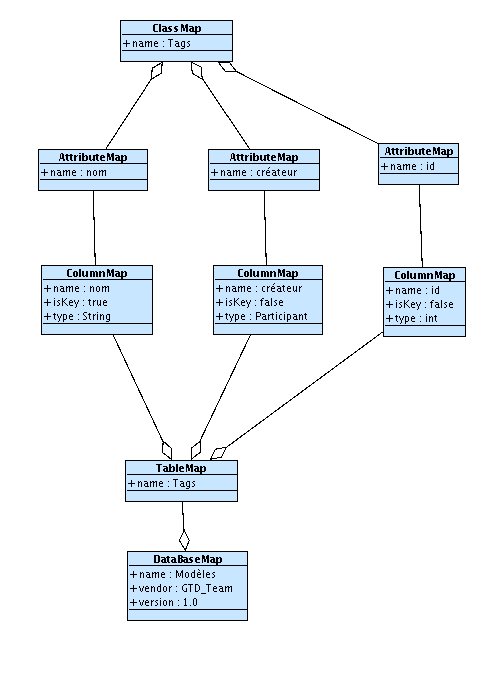
\includegraphics[width=14cm]{images/L4/TagsDBS.png}
	\caption{Schéma de la base de données : Table Tags}
	\label{TagDBS}
\end{figure}


\begin{figure}[htbp]

		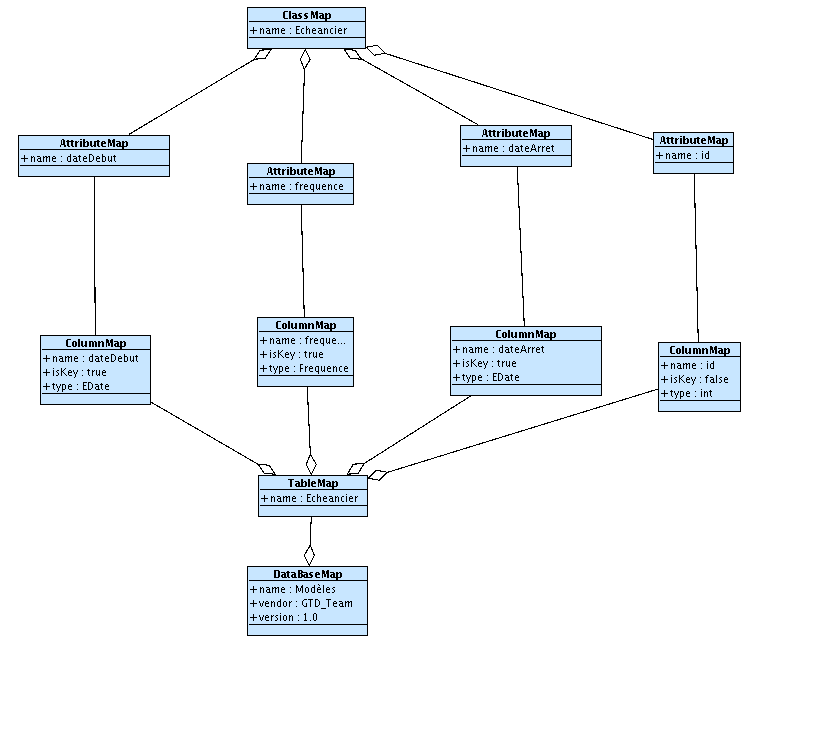
\includegraphics[width=18cm]{images/L4/EcheancierDBS.png}
	\caption{Schéma de la base de données : Table Echeancier}
	\label{EcheancierDBS}
\end{figure}


\begin{figure}[htbp]

		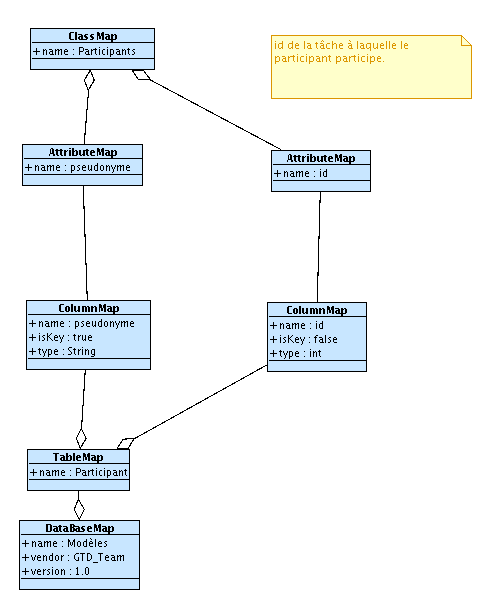
\includegraphics[width=16cm]{images/L4/ParticipantDBS.png}
	\caption{Schéma de la base de données : Table Participant}
	\label{ParticipantDBS}
\end{figure}



\begin{figure}[htbp]

		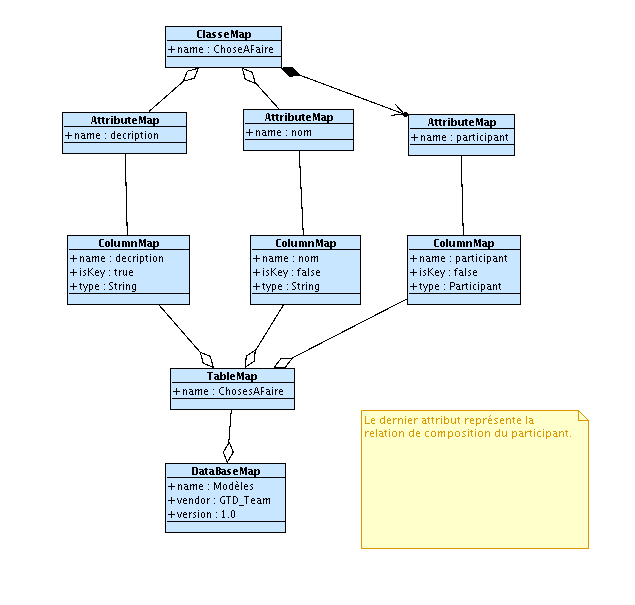
\includegraphics[width=18cm]{images/L4/ChoseDBS.png}
	\caption{Schéma de la base de données : Table Chose à faire}
	\label{ChoseDBS}
\end{figure}
A la différence des tables précédentes, la table "ChoseAFaire" \ref{ChoseDBS} contient une colonne pour mémoriser le participant de l'action (il peut ne pas y en avoir).\\

\paragraph*{}
Puis on termine par les classes héritant d'attributs communs provenant de la classe "Élément" :\\

\begin{figure}[htbp]

		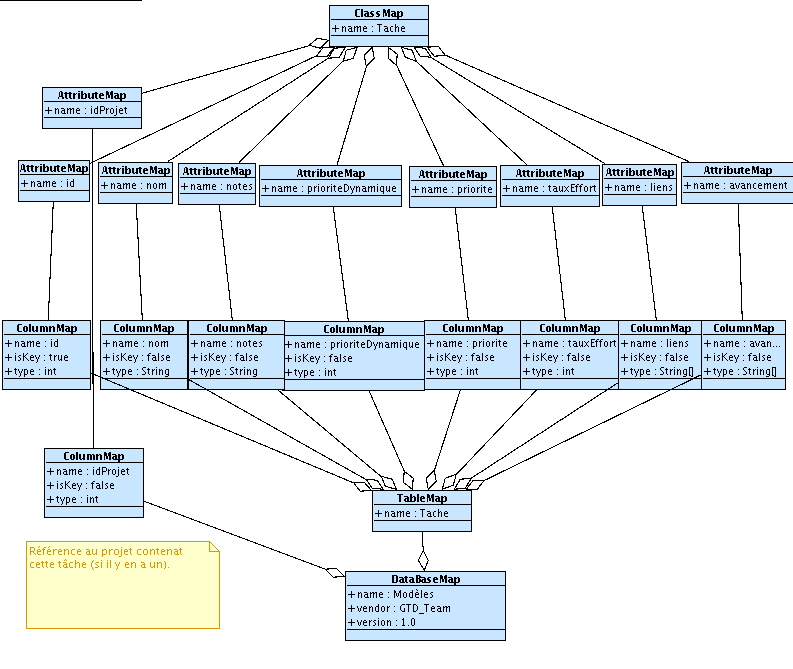
\includegraphics[width=18cm]{images/L4/TacheDBS.png}
	\caption{Schéma de la base de données : Table Tâches}
	\label{TacheDBS}
\end{figure}
\paragraph*{}
On retrouve donc dans la table "Tâche" \ref{TacheDBS} tous les attributs de la classe "Élément" et ceux de la classe "Tâche", plus un attribut référençant le projet contenant cette tâche (s'il y en a un).\\


\begin{figure}[htbp]

		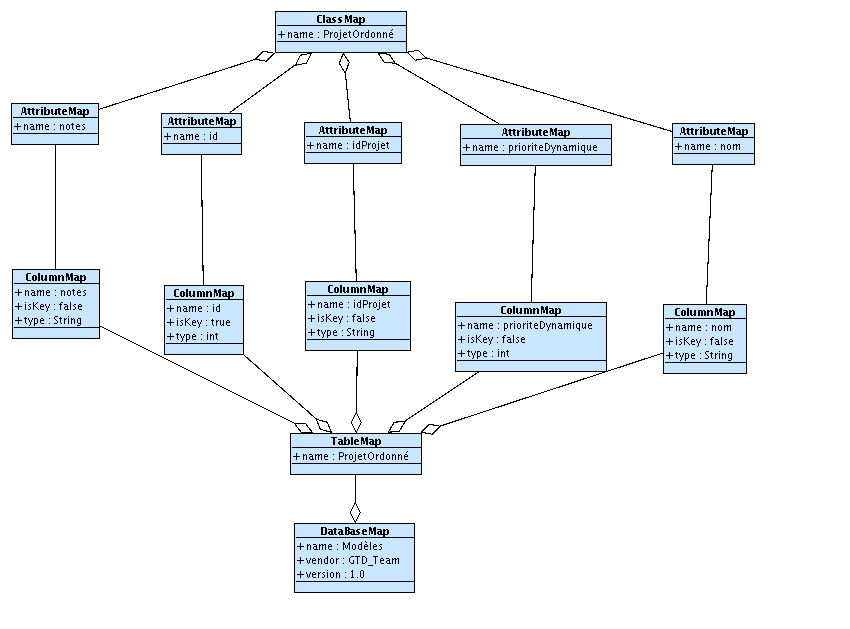
\includegraphics[width=18cm]{images/L4/ProjetNonOrdDBS.png}
	\caption{Schéma de la base de données : Table Projets Non Ordonnés}
	\label{ProjetNonOrdDBS}
\end{figure}
\paragraph*{}
De même pour un "Projet Non Ordonné" \ref{ProjetNonOrdDBS} qui peut être le sous-projet d'un autre projet.\\


\begin{figure}[htbp]

		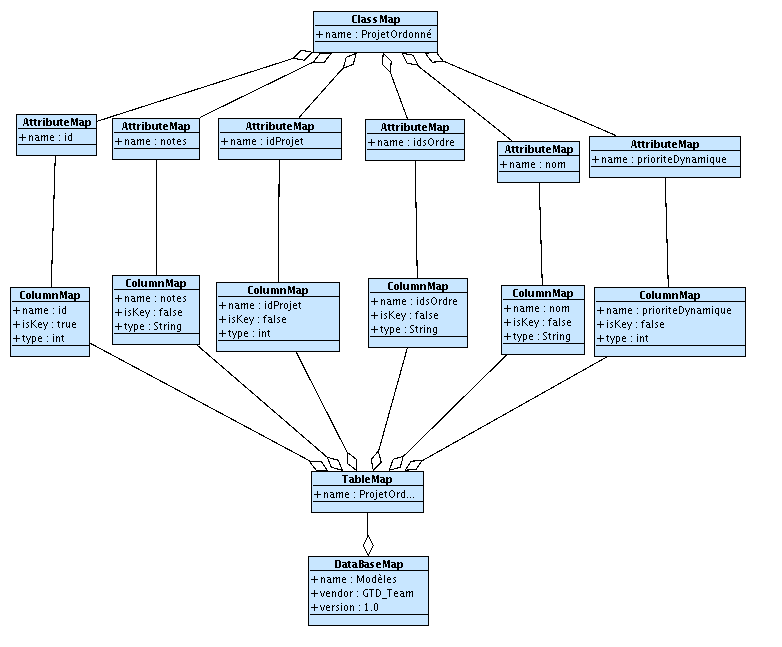
\includegraphics[width=18cm]{images/L4/ProjetOrdDBS.png}
	\caption{Schéma de la base de données : Table Projets Ordonnés}
	\label{ProjetOrdDBS}
\end{figure}
\paragraph*{}
Les "Projets Ordonnés" \ref{ProjetOrdDBS} peuvent aussi être des sous-projets mais doivent se "souvenir" de l'ordre des tâches qu'il contienne d'où la chaîne de caractères contenant les ids ordonnés des tâches d'un "Projet Ordonné".


\section{Stéréotypes et étiquettes}
Pour pouvoir implémenter proprement notre logiciel, nous avons utilisé différents patrons de conception pour créer son architecture.


	\subsection{Modèle-Vue-Contrôleur}
	Dans un premier temps, nous avons découper nos classes en 3 parties. Ce qui nous a permis d'y voir un peu plus clair dans ce que fait chaque composants logiciels. Dans notre diagramme de classes, la partie Vue n'apparaît pas car elle est plus extérieure; mais elle est bien présente dans notre logiciel. 
	
	\subsection{Projets : patron Composite}
	Selon notre diagramme de classes, un Projet est un Élément. Seulement nous avons défini depuis le début qu'un Projet peut contenir des sous-Projets; c'est pourquoi nous avons utilisé ici le patron Composite.
	
	\subsection{Méthode GTD : patron Stratégie}
	La partie Organisation de la méthode GTD est une partie complexe et nous avons choisi d'utiliser le patron Stratégie pour pouvoir changer facilement son code. Ce qui nous donne la possibilité de changer cette méthode à tout moment pour l'améliorer ou changer complètement son code métier.
	
	\subsection{Comptes : patron Visiteur}
	On utilise le patron Visiteur pour pouvoir accéder facilement au différentes valeurs stockées dans le Modèle.
	


\section{Règles de traduction}

On utilise les règles suivantes de traduction de l'UML vers Java avec Acceleo:
\begin{itemize}
\item Chaque package  dans le diagramme de classe se transforme en \textit{Package Java};
\item Chaque classe génère une \textit{Class Java} ainsi que son constructeur;
\item Chaque interface génère des \textit{Interfaces Java};
\item Une propriété donne une méthode;
\item Un attribut est privé et on génère des \textit{Getters/Setters};
\item Pour les attributs avec une multiplicité supérieur, on place l'attribut Java dans une \textit{LinkedList} et on ajoute des méthodes d'ajout et de suppression dans cette liste;
\item Si une classe hérite d'une autre, on rajoute le \textit{extend};
\item Une classe qui implémente une interface se voit ajouter \textit{implements}et on génère les méthodes de l'interface que la classe implémente.
\end{itemize}

\paragraph*{}
Ces quelques règles nous permettent de générer du code sur lequel nous pourrons "greffer" le code métier de notre application.

\section*{Conclusion}
Puisque nous avons défini l'architecture globale de notre logiciel, nous pouvons dès à présent nous intéresser aux détails des composants et ainsi définir tous les détails précédant la partie de codage visant à remplir le code généré.


	
	
	
	